\documentclass[notitlepage]{report}
\usepackage{amsmath,amsfonts,amsthm,amssymb}
\usepackage{authblk}
\usepackage[T1]{fontenc}
\usepackage{graphicx}
\usepackage[utf8]{inputenc}
\usepackage[UTF8]{ctex}
\usepackage[framemethod=tikz]{mdframed}
\usepackage{natbib}
\usepackage{subcaption}
\usepackage{tikz}
\usepackage{xcolor}
\usepackage{epigraph}
\usepackage{float}

\usepackage{hyperref}


\definecolor{blue}{RGB}{38,139,210}
\definecolor{cyan}{RGB}{42,161,152}
\definecolor{violet}{RGB}{108,113,196}
\definecolor{red}{RGB}{220,50,47}
\definecolor{base01}{RGB}{88,110,117}
\definecolor{base02}{RGB}{7,54,66}
\definecolor{base03}{RGB}{0,43,54}

\usetikzlibrary{calc,shapes,positioning}

\newcommand{\todo}[1]{\textcolor{red}{TODO: #1}}

\newtheorem{relationship}{Relationship}
\providecommand*{\relationshipautorefname}{Relationship}
\surroundwithmdframed[
    topline=false,
    bottomline=false,
    middlelinewidth=0.5pt,
    linecolor=base01,
    roundcorner=5pt,
    innertopmargin=0pt,
    leftmargin=15pt,
    rightmargin=15pt,
    nobreak=true,
]{relationship}

\setcounter{MaxMatrixCols}{16}

\let\originalepigraph\epigraph
\renewcommand\epigraph[2]{\originalepigraph{\textit{#1}}{\textsc{#2}}}

% Use arabic numbers for thanks
\makeatletter
\let\@fnsymbol\@arabic
\makeatother

\title{深度学习卷积算法指南}
\author[$\bigstar$]{Vincent Dumoulin\thanks{dumouliv@iro.umontreal.ca}}
\author[$\bigstar\dagger$]{Francesco Visin\thanks{francesco.visin@polimi.it}}
\affil[$\bigstar$]{MILA, Universit\'{e} de Montr\'{e}al}
\affil[$\dagger$]{AIRLab, Politecnico di Milano}
\date{\today}

\begin{document}

\maketitle
\thispagestyle{empty}
\clearpage

\setlength{\epigraphwidth}{0.4\textwidth}
\epigraph{All models are wrong, but some are useful.}{George E. P. Box}
\clearpage

\renewcommand{\abstractname}{Acknowledgements}
\begin{abstract}
    The authors of this guide would like to thank David Warde-Farley, Guillaume
    Alain and Caglar Gulcehre for their valuable feedback. We are likewise
    grateful to all those who helped improve this tutorial with helpful
    comments, constructive criticisms and code contributions. Keep them coming!

    Special thanks to Ethan Schoonover, creator of the Solarized color
    scheme,\footnote{\url{http://ethanschoonover.com/solarized}} whose colors
    were used for the figures.
\end{abstract}

\renewcommand{\abstractname}{Feedback}
\begin{abstract}
    Your feedback is welcomed! We did our best to be as precise, informative and
    up to the point as possible, but should there be anything you feel might be
    an error or could be rephrased to be more precise or comprehensible, please
    don't refrain from contacting us. Likewise, drop us a line if you think
    there is something that might fit this technical report and you would like
    us to discuss -- we will make our best effort to update this document.
\end{abstract}

\renewcommand{\abstractname}{Source code and animations}
\begin{abstract}
    The code used to generate this guide along with its figures is available on
    GitHub.\footnote{\url{https://github.com/vdumoulin/conv_arithmetic}} There
    the reader can also find an animated version of the figures.
\end{abstract}

\tableofcontents

\chapter{简介}

深度卷积神经网络(CNN)一直是深度学习取得巨大进步的核心。 虽然CNN最早在九十年代被用于解决字符识别任务
\citep{le1997reading}, 但是他们目前的广泛的应用却是由于近年来的一些工作:在2012年的ImageNet图像分类
挑战中一个深度神经网络模型击败了当时的最好的方案\citep{krizhevsky2012imagenet}。

因此卷积神经网络构成了一个对于机器学习学习者的一个非常有用的工具。然而第一次学习使用卷积通常都是整个人
都是懵逼的状态。卷积层的输出大小受输入大小以及卷积核大小、填充方式、以及步长的选择,而他们之间的关系又
不是那么容易推断。这核全连接层的有很大不同,因为全连接层的输出形状与输入是完全独立的。除此之外,相对于
全连接层,卷积层的{\em pooling \/}的阶段又增加了卷积操作的复杂度。最后,采用了所谓的转置卷积层(也称
为微步卷积)到目前为止,越来越多的工作和他们的工作已经不同程度地清晰地解释了转置卷积与卷积的关系fractionally 
strided convolutional layers\citep{zeiler2011adaptive,zeiler2014visualizing,
long2015fully,radford2015unsupervised,visin15,im2016generating}。

本指南的目标主要有两方面:
\begin{enumerate}
    \item 尽可能解释清楚卷积层与转置卷积层之间的关系。
    \item 在卷积操作、pooling操作以及转置卷积操作中,关于输入大小、卷积核大小、填充方式、步长与输出大
          小之间的关系以更加直观的理解方式呈现出来。
\end{enumerate}

为了保证应用的广泛性,本指南所展示的实验结果独立于具体实现细节,并且适用于所有通用的机
器学习框架图Theano\citep{bergstra2010theano,bastien2012theano},
Torch \citep{collobert2011torch7},
Tensorflow \citep{abaditensorflow} and Caffe \citep{jia2014caffe}等。

本章简要回顾了卷积神经网络的主要构成模块,即离散卷积和pooling。欲更加深入了解该相关课题,
可以参看深度学习经典教材<<Deep learning>>的第九章\citep{Goodfellow-et-al-2016-Book}。

\section{离散卷积}
神经网络的基本功能是进行\emph{仿射变换(affine transformations)}:接收一个向量作为输入并将其与矩阵进行相
乘以产生输出(在将输出进行非线性映射之前,都会给将其加上一个偏置向量)。输入可以是任意类型的,
可以是一张图片,可以是一段声音,可以是无序的特征片段,在进行输入之前这些数据总可以被表示成向量。

图片、声音片段以及其他类似数据类型都有内在结构,更准确的说,他们都具有以下属性:

\begin{itemize}
    \item 它们都以多维数组的形式进行存储。
    \item 它们具有一个或多个轴,并且每个轴上的数据的顺序很重要。(如图片的长度和高度、声音片段的时间
          等)。
    \item 一个轴被称作通道轴,用于访问数据的不同视图。(彩色图片的 R、G、B通道,立体声轨的左右通道)。
\end{itemize}

当对数据进行仿射变换时这些特征并没有利用到。实际上,所有轴上的数据都以相同的处理方式对待,像拓扑信息
这些并没有被考虑进去。因此,如果利用数据的这种隐含的结构可能会为解决譬如计算机视觉、语音识别等问题提
供方便,在这种情况下,数据的拓扑信息最好被保留下来。基于此,离散卷积应运而生。

离散卷积是一种保留了数据顺序信息的线性运算。它是稀疏的(只有少数的输入单元参与给定的输出单元的计算)。
它是参数重用的(相同的权重参数被输入的多个位置重用)。

\autoref{fig:numerical_no_padding_no_strides} 提供了一个离散卷积的例子,淡蓝色网格被称作
{\em 输入特征图(input feature map)}. 为了绘图方便,图示只展示了单个的输入特征图,但是多
个特征图堆叠的例子也是很常见的\footnote{%
    相关例子见前面所提到的图片和声音片段的{\em 通道(channels)\/}。}
一个带有参数的 {\em 卷积核(kernel)\/} (阴影区域)在输入的特征图上滑动。在每一个位置上,卷积核和输入
特征图重叠的每个元素分别进行相乘,并将相乘的结果进行求和作为当前对应位置的输出。这个过程可以按照自己
所需要的输出特征图数目来利用不同的卷积核进行多次重复操作。 (\autoref{fig:full_picture}). 该步骤的
最终输出被称作为{\em 输出特征图}.\footnote{%
    尽管互从信号处理的角度来看互相关和卷积有一定的区别  ,但是当学习内核时,这两个概念是可以互相交换的。
    为了方便以及与大部分的机器学习文献保持一致,本指南中将使用{\em 卷积\/}一词。
}

\begin{figure}[H]
    \centering
    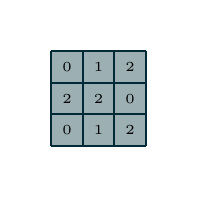
\begin{tikzpicture}[scale=.4,every node/.style={minimum size=1cm}, on grid]
            \draw[fill=base02,opacity=0.4] (0,0) rectangle (3,3);
            \draw[draw=base03,thick] (0,0) grid (3,3);
            \node (00) at (0.5,2.5) {\tiny 0};
            \node (01) at (1.5,2.5) {\tiny 1};
            \node (02) at (2.5,2.5) {\tiny 2};
            \node (10) at (0.5,1.5) {\tiny 2};
            \node (11) at (1.5,1.5) {\tiny 2};
            \node (12) at (2.5,1.5) {\tiny 0};
            \node (20) at (0.5,0.5) {\tiny 0};
            \node (21) at (1.5,0.5) {\tiny 1};
            \node (22) at (2.5,0.5) {\tiny 2};
    \end{tikzpicture}
\end{figure}

\begin{figure}[p]
    \centering
    \includegraphics[width=0.32\textwidth]{pdf/numerical_no_padding_no_strides_00.pdf}
    \includegraphics[width=0.32\textwidth]{pdf/numerical_no_padding_no_strides_01.pdf}
    \includegraphics[width=0.32\textwidth]{pdf/numerical_no_padding_no_strides_02.pdf}
    \includegraphics[width=0.32\textwidth]{pdf/numerical_no_padding_no_strides_03.pdf}
    \includegraphics[width=0.32\textwidth]{pdf/numerical_no_padding_no_strides_04.pdf}
    \includegraphics[width=0.32\textwidth]{pdf/numerical_no_padding_no_strides_05.pdf}
    \includegraphics[width=0.32\textwidth]{pdf/numerical_no_padding_no_strides_06.pdf}
    \includegraphics[width=0.32\textwidth]{pdf/numerical_no_padding_no_strides_07.pdf}
    \includegraphics[width=0.32\textwidth]{pdf/numerical_no_padding_no_strides_08.pdf}
    \caption{\label{fig:numerical_no_padding_no_strides}计算离散卷积的输出值。}
\end{figure}

\begin{figure}[p]
    \centering
    \includegraphics[width=0.32\textwidth]{pdf/numerical_padding_strides_00.pdf}
    \includegraphics[width=0.32\textwidth]{pdf/numerical_padding_strides_01.pdf}
    \includegraphics[width=0.32\textwidth]{pdf/numerical_padding_strides_02.pdf}
    \includegraphics[width=0.32\textwidth]{pdf/numerical_padding_strides_03.pdf}
    \includegraphics[width=0.32\textwidth]{pdf/numerical_padding_strides_04.pdf}
    \includegraphics[width=0.32\textwidth]{pdf/numerical_padding_strides_05.pdf}
    \includegraphics[width=0.32\textwidth]{pdf/numerical_padding_strides_06.pdf}
    \includegraphics[width=0.32\textwidth]{pdf/numerical_padding_strides_07.pdf}
    \includegraphics[width=0.32\textwidth]{pdf/numerical_padding_strides_08.pdf}
    \caption{\label{fig:numerical_padding_strides} 计算参数为 $N = 2$, $i_1 = i_2 = 5$, $k_1 = k_2 = 3$,
        $s_1 = s_2 = 2$, 以及 $p_1 = p_2 = 1$时的离散卷积输出值。}
\end{figure}

如果输入多个特征图,则卷积核的数目必须是3维的。类似的,每个特征图都会与不同的卷积核分别进行
卷积操作生成不同的特征图,这些生成的特征图对应位置元素相加形成一个新的特征图。

图\autoref{fig:numerical_no_padding_no_strides}所展示的卷积是一个二维卷积的例子,但是它
可以推广到N维卷积的情形。比如,在三维卷积中,卷积核将会是一个{\em 立方体\/},并且它将从输入
特征图的长、宽、高、三个维度进行滑动。

定义离散卷积的众多卷积核的集合的尺寸主要和这些元素有关$(n, m, k_1, \ldots, k_N)$,
其中

\begin{equation*}
\begin{split}
    n &\equiv \text{输出特征图数目},\\
    m &\equiv \text{输入特征图数目},\\
    k_j &\equiv \text{沿 $j$轴 的卷积核尺寸}.
\end{split}
\end{equation*}

以下参数影响卷积层在 $j$ 轴的输出尺寸:


\begin{itemize}
    \item $i_j$: 沿 $j$ 轴的输入尺寸,
    \item $k_j$: 沿 $j$ 轴的卷积核尺寸,
    \item $s_j$: 沿 $j$ 轴的步长(内核在特征图上每次进行滑动的距离),
    \item $p_j$: 沿 $j$轴的0填充(在某一维上从开始到结束时填充0)数目.
\end{itemize}

\noindent例图\autoref{fig:numerical_padding_strides} 展现了一个 $3
\times 3$ 大小的卷积核在输入特征图为 $5 \times 5$、边界0填充为$1 \times 1$
步长为 $2 \times 2$ 时进行卷积的情形。

注意到步长构成了一种\emph{子采样}的形式。作为解释卷积核参与变换的度量参数,步长也可
以被看做多少输出被保存下来。比如,在对卷积核进行步长为2的滑动时和进行步长为1的滑动但
是仅仅保存奇数位输出是等效的(\autoref{fig:strides_subsampling})。


\begin{figure}[p]
    \centering
    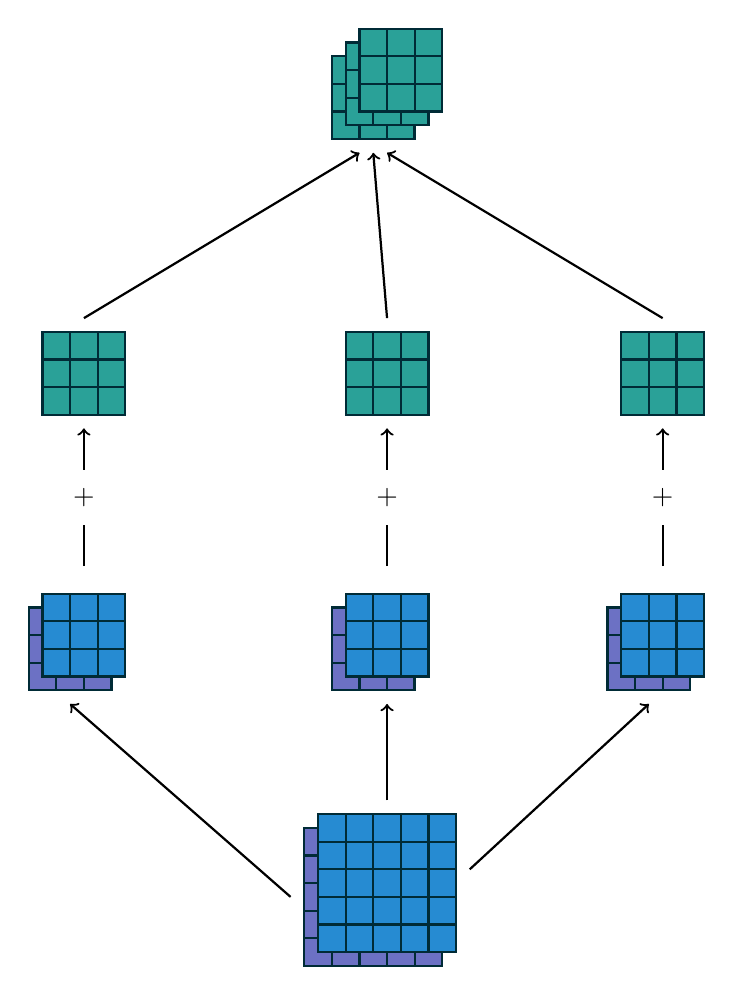
\begin{tikzpicture}[scale=.35,every node/.style={minimum size=1cm}, on grid]
        \begin{scope}[xshift=0cm,yshift=0cm]
            \begin{scope}[xshift=0cm,yshift=0cm]
                \draw[draw=base03,fill=violet,thick]
                    (0,0) grid (5,5) rectangle (0,0);
            \end{scope}
            \begin{scope}[xshift=0.5cm,yshift=0.5cm]
                \draw[draw=base03,fill=blue,thick]
                    (0,0) grid (5,5) rectangle (0,0);
            \end{scope}
        \end{scope}
        \foreach \x in {-10,1,11} {%
            \begin{scope}[xshift=\x cm,yshift=10cm]
                \begin{scope}[xshift=0cm,yshift=0cm]
                    \draw[draw=base03,fill=violet,thick]
                        (0,0) grid (3,3) rectangle (0,0);
                \end{scope}
                \begin{scope}[xshift=0.5cm,yshift=0.5cm]
                    \draw[draw=base03,fill=blue,thick]
                        (0,0) grid (3,3) rectangle (0,0);
                \end{scope}
            \end{scope}
            \begin{scope}[xshift=\x cm,yshift=20cm]\begin{scope}[xshift=0.5cm]
                \draw[draw=base03,fill=cyan,thick]
                    (0,0) grid (3,3) rectangle (0,0);
            \end{scope}\end{scope}
        }
        \begin{scope}[xshift=1cm,yshift=30cm]
            \foreach \s in {0.0,0.5,1.0} {%
                \begin{scope}[xshift=\s cm,yshift=\s cm]
                    \draw[draw=base03,fill=cyan,thick]
                        (0,0) grid (3,3) rectangle (0,0);
                \end{scope}
            }
        \end{scope}
        \draw[->, thick] (-0.5,2.5) to (-8.5,9.5);
        \draw[->, thick] (3,6) to (3,9.5);
        \draw[->, thick] (6,3.5) to (12.5,9.5);
        \draw[thick]  (-8,14.5) to (-8,16);
        \draw[->, thick]  (-8,18) to (-8,19.5);
        \node[thick] (p1) at (-8,17) {$+$};
        \draw[thick]  (3,14.5) to (3,16);
        \draw[->, thick]  (3,18) to (3,19.5);
        \node[thick] (p2) at (3,17) {$+$};
        \draw[thick]  (13,14.5) to (13,16);
        \draw[->, thick]  (13,18) to (13,19.5);
        \node[thick] (p3) at (13,17) {$+$};
        \draw[->, thick]  (-8,23.5) to (2,29.5);
        \draw[->, thick]  (3,23.5) to (2.5,29.5);
        \draw[->, thick]  (13,23.5) to (3,29.5);
    \end{tikzpicture}

    \caption{\label{fig:full_picture} 展示了从一个特征图数目为2作为输入,通过使用$3 \times 2 \times 3
    \times 3$的卷积核$\mathbf{w}$进行映射使输出特征图数目变为3的例子。在示意图的左半侧,输入特征图1和和
    卷积核$\mathbf{w}_{1,1}$进行卷积,特征图2和卷积核$\mathbf{w}_{1,2}$进行卷积,然后将以上两次卷积的
    输出的对应位置元素进行相加求和即可得到新的特征图。在图示中间部分以及右部重复以上操作将会分别产生第二、
    第三张特征图,把所有的输出特征图进行组合即可得到新的输出。
    }

\end{figure}

\begin{figure}[p]
    \centering
    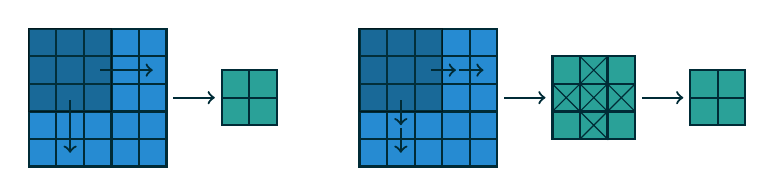
\begin{tikzpicture}[scale=.35,every node/.style={minimum size=1cm}, on grid]
        \begin{scope}[xshift=0,yshift=0cm]
            \begin{scope}[xshift=0cm,yshift=0cm]
                \draw[draw=base03,fill=blue,thick] (0,0) grid (5,5) rectangle (0,0);
                \draw[fill=base02, opacity=0.4] (0,2) rectangle (3,5);
            \end{scope}
            \begin{scope}[xshift=7cm,yshift=1.5cm]
                \draw[draw=base03,fill=cyan,thick] (0,0) grid (2,2) rectangle (0,0);
            \end{scope}
        \end{scope}
        \draw[draw=base03, ->, thick] (2.6,3.5) to  (4.5,3.5);
        \draw[draw=base03, ->, thick] (1.5,2.4) to (1.5,0.5);
        \draw[draw=base03, ->, thick] (5.25, 2.5) to (6.75, 2.5);
        \begin{scope}[xshift=12cm,yshift=0cm]
            \begin{scope}[xshift=0cm,yshift=0cm]
                \draw[draw=base03,fill=blue,thick] (0,0) grid (5,5) rectangle (0,0);
                \draw[fill=base02, opacity=0.4] (0,2) rectangle (3,5);
            \end{scope}
            \begin{scope}[xshift=7cm,yshift=1cm]
                \draw[draw=base03,fill=cyan,thick] (0,0) grid (3,3) rectangle (0,0);
                \draw[draw=base03] (1,0) -- (2,1) -- (2,0) -- (1,1);
                \draw[draw=base03] (0,1) -- (1,2) -- (1,1) -- (0,2);
                \draw[draw=base03] (1,1) -- (2,2) -- (2,1) -- (1,2);
                \draw[draw=base03] (2,1) -- (3,2) -- (3,1) -- (2,2);
                \draw[draw=base03] (1,2) -- (2,3) -- (2,2) -- (1,3);
            \end{scope}
            \begin{scope}[xshift=12cm,yshift=1.5cm]
                \draw[draw=base03,fill=cyan,thick] (0,0) grid (2,2) rectangle (0,0);
            \end{scope}
        \end{scope}
        \draw[draw=base03, ->, thick] (14.6,3.5) to  (15.5,3.5);
        \draw[draw=base03, ->, thick] (15.6,3.5) to  (16.5,3.5);
        \draw[draw=base03, ->, thick] (13.5,2.4) to (13.5,1.5);
        \draw[draw=base03, ->, thick] (13.5,1.4) to (13.5,0.5);
        \draw[draw=base03, ->, thick] (17.25, 2.5) to (18.75, 2.5);
        \draw[draw=base03, ->, thick] (22.25, 2.5) to (23.75, 2.5);
    \end{tikzpicture}
    \caption{\label{fig:strides_subsampling} 另外一种审视步长的角度:不再用将$3 \times 3$卷积核解读为滑动
    增量为2$s = 2$ (左图),而是将其解读为滑动增量为1但是只保存$s = 2$时的元素输出(右图)。}
\end{figure}

\section{池化}

除了离散卷积本身, {\em 池化\/}操作也是卷积神经网络的重要组成模块。池化操作通过使用一些函数来
对特征图的某个区域进行摘要提取来实现对输入特征图的降维,常用的操作比如取某一池化区域的最大值
或者均值。

池化通过在输入的特征图上进行滑动并且根据{\em 池化函数}来进行窗口数据的填充。在某些情景下,池化
的工作方式和离散卷积特别像,只是将卷积核的线性组合方式变成了一些其他的函数。
\autoref{fig:numerical_average_pooling}展示了平均池化的例子,\autoref{fig:numerical_max_pooling}
展示了最大值池化的例子。

以下参数影响池化层在$j$轴的输出尺寸$o_j$:

\begin{itemize}
    \item $i_j$: 沿 $j$轴的输入尺寸,
    \item $k_j$: 沿 $j$轴的池化窗口大小。
    \item $s_j$: 沿 $j$轴的步长(池化窗口在特征图上的滑动距离)。
\end{itemize}

\begin{figure}[p]
    \centering
    \includegraphics[width=0.32\textwidth]{pdf/numerical_average_pooling_00.pdf}
    \includegraphics[width=0.32\textwidth]{pdf/numerical_average_pooling_01.pdf}
    \includegraphics[width=0.32\textwidth]{pdf/numerical_average_pooling_02.pdf}
    \includegraphics[width=0.32\textwidth]{pdf/numerical_average_pooling_03.pdf}
    \includegraphics[width=0.32\textwidth]{pdf/numerical_average_pooling_04.pdf}
    \includegraphics[width=0.32\textwidth]{pdf/numerical_average_pooling_05.pdf}
    \includegraphics[width=0.32\textwidth]{pdf/numerical_average_pooling_06.pdf}
    \includegraphics[width=0.32\textwidth]{pdf/numerical_average_pooling_07.pdf}
    \includegraphics[width=0.32\textwidth]{pdf/numerical_average_pooling_08.pdf}
    \caption{\label{fig:numerical_average_pooling} Computing the output values
        of a $3 \times 3$ average pooling operation on a $5 \times 5$ input
        using $1 \times 1$ strides.}
\end{figure}

\begin{figure}[p]
    \centering
    \includegraphics[width=0.32\textwidth]{pdf/numerical_max_pooling_00.pdf}
    \includegraphics[width=0.32\textwidth]{pdf/numerical_max_pooling_01.pdf}
    \includegraphics[width=0.32\textwidth]{pdf/numerical_max_pooling_02.pdf}
    \includegraphics[width=0.32\textwidth]{pdf/numerical_max_pooling_03.pdf}
    \includegraphics[width=0.32\textwidth]{pdf/numerical_max_pooling_04.pdf}
    \includegraphics[width=0.32\textwidth]{pdf/numerical_max_pooling_05.pdf}
    \includegraphics[width=0.32\textwidth]{pdf/numerical_max_pooling_06.pdf}
    \includegraphics[width=0.32\textwidth]{pdf/numerical_max_pooling_07.pdf}
    \includegraphics[width=0.32\textwidth]{pdf/numerical_max_pooling_08.pdf}
    \caption{\label{fig:numerical_max_pooling}在$5 \times 5$的输入特征图上进行$3 \times 3$且步长为
    $1 \times 1$最大值池化操作。}
\end{figure}

\chapter{卷积算法}

由于卷积层参数之间不会跨轴进行交互,因此关于他们之间关系的分析还是比较简单的。比如沿$j$轴卷积核大小、
步长、0填充等参数之后影响$j$轴的输出。因此,本章的讨论将会在以下简单设定下进行:

\begin{itemize}
    \item 二维离散卷积 ($N = 2$),
    \item 输入为正方形 ($i_1 = i_2 = i$),
    \item 卷积核尺寸为正方形 ($k_1 = k_2 = k$),
    \item 沿每个轴的步长相同 ($s_1 = s_2 = s$),
    \item 沿每个轴的0填充相同 ($p_1 = p_2 = p$).
\end{itemize}

以上假设有利于分析以及可视化,但要记住的是这里描述得到的结果同样适用于任意维度的的卷积以及
非正方形参数的情况。

\section{无0填充-单位步长}

这是分析起来最简单的一种情况:卷积核只是从输入特征图的每个位置滑过。\autoref{fig:no_padding_no_strides}
展示了$s = 1$ 、$p = 0$、$i = 4$、$k =3$的情形。


在这种情形下,一种定义输出尺寸的方式是根据卷积核在输入特征图上的可以到达的位置数目。沿输入特征图的宽度举例:
卷积核在输入特征图的最左侧开始滑动直到到达输入特征图的最右侧的边,并且每次滑动的距离为一个单位。输出的尺寸
大小将等于滑动的步数加1(1为卷积核最开始的所处的位置)(\autoref{fig:no_padding_no_strides_explained}。
在沿着输入特征图高度进行滑动时是同样的逻辑。

更准确的说,可以推断出以下关系式:

\begin{relationship}\label{rel:no_padding_no_strides}
For any $i$ and $k$, and for $s = 1$ and $p = 0$,
\begin{equation*}
    o = (i - k) + 1.
\end{equation*}
\end{relationship}

\begin{figure}[p]
    \centering
    \includegraphics[width=0.24\textwidth]{pdf/no_padding_no_strides_00.pdf}
    \includegraphics[width=0.24\textwidth]{pdf/no_padding_no_strides_01.pdf}
    \includegraphics[width=0.24\textwidth]{pdf/no_padding_no_strides_02.pdf}
    \includegraphics[width=0.24\textwidth]{pdf/no_padding_no_strides_03.pdf}
    \caption{\label{fig:no_padding_no_strides} (无0填充-单位步长)
        $3 \times 3$的卷积核在$4 \times 4$的输入特征图上以单位步长进行卷积(即$i = 4$, $k = 3$, 
        $s = 1$ 以及 $p = 0$)。
        }
\end{figure}

\begin{figure}[p]
    \centering
    \includegraphics[width=0.24\textwidth]{pdf/arbitrary_padding_no_strides_00.pdf}
    \includegraphics[width=0.24\textwidth]{pdf/arbitrary_padding_no_strides_01.pdf}
    \includegraphics[width=0.24\textwidth]{pdf/arbitrary_padding_no_strides_02.pdf}
    \includegraphics[width=0.24\textwidth]{pdf/arbitrary_padding_no_strides_03.pdf}
    \caption{\label{fig:arbitrary_padding_no_strides} (任意填充-单位步长)
        $4 \times 4$的卷积核以单位步长在$2 \times 2$0填充的$5 \times 5$的输入特征图上进行卷积。
        (即$i = 5$, $k = 4$, $s = 1$ 以及 $p = 2$)。
        }
\end{figure}

\begin{figure}[p]
    \centering
    \includegraphics[width=0.24\textwidth]{pdf/same_padding_no_strides_00.pdf}
    \includegraphics[width=0.24\textwidth]{pdf/same_padding_no_strides_01.pdf}
    \includegraphics[width=0.24\textwidth]{pdf/same_padding_no_strides_02.pdf}
    \includegraphics[width=0.24\textwidth]{pdf/same_padding_no_strides_03.pdf}
    \caption{\label{fig:same_padding_no_strides} (半填充-单位步长)
        $3 \times 3$的卷积核以单位步长在半填充的$5 \times 5$的输入特征图上进行卷积。
        (即$i = 5$, $k = 3$, $s = 1$ 以及 $p = 1$)。
    }
\end{figure}

\begin{figure}[p]
    \centering
    \includegraphics[width=0.24\textwidth]{pdf/full_padding_no_strides_00.pdf}
    \includegraphics[width=0.24\textwidth]{pdf/full_padding_no_strides_01.pdf}
    \includegraphics[width=0.24\textwidth]{pdf/full_padding_no_strides_02.pdf}
    \includegraphics[width=0.24\textwidth]{pdf/full_padding_no_strides_03.pdf}
    \caption{\label{fig:full_padding_no_strides} (全填充-单位步长)
        Convolving a $3 \times 3$ kernel over a $5 \times 5$ input using full
        padding and unit strides (i.e., $i = 5$, $k = 3$, $s = 1$ and $p = 2$).}
\end{figure}

\section{有0填充-单位步长}

我们来考虑一下$s = 1$时0填充对有效输入的影响:填充$p$个0把有效输入的尺寸由 $i$变为$i + 2p$。
在该情形下,由\autoref{rel:no_padding_no_strides}可以推出以下关系式:


\begin{relationship}\label{rel:arbitrary_padding_no_strides}
对任意的 $i$, $k$ , $p$, 当 $s = 1$时,
\begin{equation*}
    o = (i - k) + 2p + 1.
\end{equation*}
\end{relationship}

\noindent \autoref{fig:arbitrary_padding_no_strides} 展示了 $i
= 5$, $k = 4$ , $p = 2$的例子。

\noindent \autoref{fig:arbitrary_padding_no_strides} provides an example for $i
= 5$, $k = 4$ and $p = 2$.

在实际操作中,有两种0填充的实例由于他们的不同特性被广泛使用。我们将在下面详细讨论.

\subsection{Half (same) padding}

输出的尺寸大小和输入相同($o = i$)是该填充方式一个比较令人期待的性质。


\begin{relationship}\label{rel:same_padding_no_strides}
对任意的 $i$ 、 $k$($k = 2n + 1, \quad n \in \mathbb{N}$)、 $s = 1$ 和
$p = \lfloor k / 2 \rfloor = n$,
\begin{equation*}
\begin{split}
    o &= i + 2 \lfloor k / 2 \rfloor - (k - 1) \\
      &= i + 2n - 2n \\
      &= i.
\end{split}
\end{equation*}
\end{relationship}


\noindent 该填充方式有时被称为半填充。图\autoref{fig:same_padding_no_strides} 展示了
$i = 5$, $k = 3$, $p = 1$时的情形。

\subsection{全填充}

卷积操作通常会{\em 减小\/}输入尺寸,但是有时我们并不想这样。在这种情况下,通过合适的0填充方式可以
达到我们的目的。

While convolving a kernel generally {\em decreases\/} the output size with
respect to the input size, sometimes the opposite is required. This can be
achieved with proper zero padding:

\begin{relationship}\label{rel:full_padding_no_strides}
对任意的 $i$ 、$k$, 以及 $p = k - 1$ 、 $s = 1$,
\begin{equation*}
\begin{split}
    o &= i + 2(k - 1) - (k - 1) \\
      &= i + (k - 1).
\end{split}
\end{equation*}
\end{relationship}

\noindent 该填充方式有时被称作 {\em 全填充\/} ,因为在此情况下卷积核在特征图上所滑过的每一个可能的部分
或者完全叠加的部分都被考虑了进去。图\autoref{fig:full_padding_no_strides}给出了
$i = 5$,$k = 3$ ,$p = 2$时的情形。

\section{无0填充-非单位步长}

迄今为止得到的关系式只适用于单位步长的卷积。非单位步进步长的的卷积输出尺寸计算和单位步进步长的计算还是有
很大区别的。为了便于分析,我们暂时不考虑0填充(即 $s > 1$、$p = 0$的情况)。 
图\autoref{fig:no_padding_strides}展示了$i =5$, $k = 3$ , $s = 2$,$s = 2$时的情形。

在此再提一下,输出尺寸可以由卷积核在输入特征图上的可能位置数目来确定。沿输入特征图的宽度举例:卷积核从输入
特征图的最左部分开始滑动,但是此次不同的是每次滑动的步长为$s$直到卷积核到达输入特征图最右端。输出特征图的
尺寸同样等于卷积核滑动步数加1---考虑到卷积核最初始的位置。(\autoref{fig:no_padding_strides_explained})
。在沿着输入特征图高度进行滑动时是同样的逻辑。


基于此,可以推断出以下关系式:

\begin{relationship}\label{rel:no_padding_strides}
对任意的 $i$, $k$ , $s$, 以及 $p = 0$,
\begin{equation*}
    o = \left\lfloor \frac{i - k}{s} \right\rfloor + 1.
\end{equation*}
\end{relationship}

\noindent 向下取整函数说明了这样一个事实:卷积核在滑动的时候最后一步可能到达不了输入特征图的最右边,
一些输入可能不会参与运算。
图\autoref{fig:padding_strides_odd}展示了这一情形。

\section{0填充-非单位步长}

最常见的情形---输入特征图进行0填充并且使用卷积步长不为单位1。为便于分析,此种情形可以认为输入的尺寸
为$i + 2p$,此时与情景\autoref{rel:arbitrary_padding_no_strides}类似。

\begin{relationship}\label{rel:padding_strides}
For any $i$, $k$, $p$ and $s$,
\begin{equation*}
    o = \left\lfloor \frac{i + 2p - k}{s} \right\rfloor + 1.
\end{equation*}
\end{relationship}

\noindent 如前所述,向下取整操会使在某些情况下不同的输入尺寸产生相同的输出尺寸。 更具体的说,如果
$i + 2p - k$是 $s$的整数倍,那么对于任何输入尺寸$j = i + a, \quad a \in \{0,\ldots,s - 1\}$
都会产生相同尺寸的输出。注意这种情况仅适用于$s > 1$的情形。


图\autoref{fig:padding_strides} 展示了 $i = 5$, $k = 3$, $s = 2$
以及 $p = 1$的情形,图 \autoref{fig:padding_strides_odd} 展示了
$i = 6$, $k = 3$, $s = 2$ 以及 $p = 1$的情形. 有趣的是,尽管输入特征图尺寸不同,但是他们的输出尺
寸是相同的。虽然这不会影响{\em 卷积}的分析,然而这会使{\em 转置卷积}的分析变得复杂。

\begin{figure}[p]
    \centering
    \includegraphics[width=0.24\textwidth]{pdf/no_padding_strides_00.pdf}
    \includegraphics[width=0.24\textwidth]{pdf/no_padding_strides_01.pdf}
    \includegraphics[width=0.24\textwidth]{pdf/no_padding_strides_02.pdf}
    \includegraphics[width=0.24\textwidth]{pdf/no_padding_strides_03.pdf}
    \caption{\label{fig:no_padding_strides} (No zero padding, arbitrary
        strides) Convolving a $3 \times 3$ kernel over a $5 \times 5$ input
        using $2 \times 2$ strides (i.e., $i = 5$, $k = 3$, $s = 2$ and
        $p = 0$).}
\end{figure}

\begin{figure}[p]
    \centering
    \includegraphics[width=0.24\textwidth]{pdf/padding_strides_00.pdf}
    \includegraphics[width=0.24\textwidth]{pdf/padding_strides_01.pdf}
    \includegraphics[width=0.24\textwidth]{pdf/padding_strides_02.pdf}
    \includegraphics[width=0.24\textwidth]{pdf/padding_strides_03.pdf}
    \caption{\label{fig:padding_strides} (Arbitrary padding and strides)
        Convolving a $3 \times 3$ kernel over a $5 \times 5$ input padded with
        a $1 \times 1$ border of zeros using $2 \times 2$ strides (i.e.,
        $i = 5$, $k = 3$, $s = 2$ and $p = 1$).}
\end{figure}

\begin{figure}[p]
    \centering
    \includegraphics[width=0.24\textwidth]{pdf/padding_strides_odd_00.pdf}
    \includegraphics[width=0.24\textwidth]{pdf/padding_strides_odd_01.pdf}
    \includegraphics[width=0.24\textwidth]{pdf/padding_strides_odd_02.pdf}
    \includegraphics[width=0.24\textwidth]{pdf/padding_strides_odd_03.pdf}
    \caption{\label{fig:padding_strides_odd} (Arbitrary padding and strides)
        Convolving a $3 \times 3$ kernel over a $6 \times 6$ input padded with
        a $1 \times 1$ border of zeros using $2 \times 2$ strides (i.e.,
        $i = 6$, $k = 3$, $s = 2$ and $p = 1$). In this case, the bottom row
        and right column of the zero padded input are not covered by the
        kernel.}
\end{figure}

\begin{figure}[p]
    \centering
    \begin{subfigure}[t]{0.48\textwidth}
        \centering
        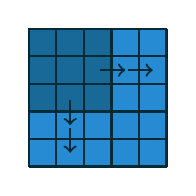
\begin{tikzpicture}[scale=.35,every node/.style={minimum size=1cm},
                            on grid]
            \draw[fill=blue] (0,0) rectangle (5,5);
            \draw[draw=base03, thick] (0,0) grid (5,5);
            \draw[fill=base02, opacity=0.4] (0,2) rectangle (3,5);
            \draw[step=10mm, base03, thick] (0,2) grid (3,5);
            \draw[draw=base03, ->, thick] (2.6,3.5) to  (3.5,3.5);
            \draw[draw=base03, ->, thick] (3.6,3.5) to  (4.5,3.5);
            \draw[draw=base03, ->, thick] (1.5,2.4) to  (1.5,1.5);
            \draw[draw=base03, ->, thick] (1.5,1.4) to  (1.5,0.5);
        \end{tikzpicture}
        \caption{\label{fig:no_padding_no_strides_explained} The kernel has to
            slide two steps to the right to touch the right side of the input
            (and equivalently downwards).  Adding one to account for the
            initial kernel position, the output size is $3 \times 3$.}
    \end{subfigure}
    ~
    \begin{subfigure}[t]{0.48\textwidth}
        \centering
        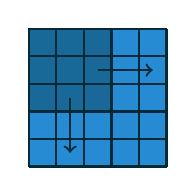
\begin{tikzpicture}[scale=.35,every node/.style={minimum size=1cm},
                            on grid]
            \draw[fill=blue] (0,0) rectangle (5,5);
            \draw[draw=base03, thick] (0,0) grid (5,5);
            \draw[fill=base02, opacity=0.4] (0,2) rectangle (3,5);
            \draw[step=10mm, base03, thick] (0,2) grid (3,5);
            \draw[draw=base03, ->, thick] (2.5,3.5) to  (4.5,3.5);
            \draw[draw=base03, ->, thick] (1.5,2.5) to  (1.5,0.5);
        \end{tikzpicture}
        \caption{\label{fig:no_padding_strides_explained} The kernel has to
            slide one step of size two to the right to touch the right side of
            the input (and equivalently downwards).  Adding one to account for
            the initial kernel position, the output size is $2 \times 2$.}
    \end{subfigure}
    \caption{Counting kernel positions.}
\end{figure}

\chapter{池化算法}

在神经网络中,池化层对小型变换提供了不变性。最常见的池化是\emph{最大值池化},基本操作时将输入特征图
(通常是非重叠的)分割成小块,然后取每个小块的最大值。其他类型的池化包括均值池化等,所有的池化方式都采
用了相同的思想:通过对输入特征图的每一小块进行非线性运算来对,最终再将这些局部输出合并
\citep{%
boureau-cvpr-10,boureau-icml-10,boureau-iccv-11,ICML2011Saxe_551}。

一些读者可能已经意识到卷积的处理只是依赖于将一些函数重复应用于输入的子集上的假设。这意味着在前一章所
推导出的关系式可以适用于池化算法。由于池化过程没有0填充参与,因此以上关系式的形式通常如下:

\begin{relationship}\label{rel:pooling}
对任意的 $i$, $k$ 以及 $s$,
\begin{equation*}
    o = \left\lfloor \frac{i - k}{s} \right\rfloor + 1.
\end{equation*}
\end{relationship}

\noindent 该关系式适用于任何池化类型。

\chapter{转置卷积算法}

转置卷积来源于对在常规卷积的相反方向应用一种变换的需求,即从某种卷积输出形状的到具有和输入具有相同
形状的变换,于此同时还能保证中间的连接模式和上述卷积兼容。比如,人们可能使用这样的变换作为卷积自编码的
解码部分或者将输入特征图映射到更高的维度上去。

再强调一遍,这种卷积情况比仅仅需要一个转置的权重矩阵的全连接的情况更加复杂。然而,由于任何卷积操作都可以
归结为矩阵运算,因此从全连接的情况得到的一些经验在解决卷积的情况是行之有效的。

与卷积算法一样,转置卷积的属性不跨轴交互的事实简化了转置卷积的讨论。

本章节将针对以下设置展开讨论:

\begin{itemize}
    \item 二维转置卷积 ($N = 2$),
    \item 输入为正方形 ($i_1 = i_2 = i$),
    \item 卷积核尺寸为正方形 ($k_1 = k_2 = k$),
    \item 沿每个轴的步长相同 ($s_1 = s_2 = s$),
    \item 沿每个轴的0填充相同 ($p_1 = p_2 = p$).
\end{itemize}

\noindent 再强调一遍,这里描述得到的结果同样适用于任意维度的的卷积以及非正方形参数的情形。

\section{卷积---作为矩阵运算}

以图\autoref{fig:no_padding_no_strides}展示的卷积为例。如果将输入和输出从左到右、从上至下展开为向量,
卷积可以用稀疏矩阵$\mathbf{C}$来表示,非零元素$w_{i,j}$是卷积核在相应位置的元素($i$、$j$ 分别分别代表
卷积核行和列的索引):

\begin{equation*}
\resizebox{.98\hsize}{!}{$
    \begin{pmatrix}
    w_{0,0} & w_{0,1} & w_{0,2} & 0       & w_{1,0} & w_{1,1} & w_{1,2} & 0       &
    w_{2,0} & w_{2,1} & w_{2,2} & 0       & 0       & 0       & 0       & 0       \\
    0       & w_{0,0} & w_{0,1} & w_{0,2} & 0       & w_{1,0} & w_{1,1} & w_{1,2} &
    0       & w_{2,0} & w_{2,1} & w_{2,2} & 0       & 0       & 0       & 0       \\
    0       & 0       & 0       & 0       & w_{0,0} & w_{0,1} & w_{0,2} & 0       &
    w_{1,0} & w_{1,1} & w_{1,2} & 0       & w_{2,0} & w_{2,1} & w_{2,2} & 0       \\
    0       & 0       & 0       & 0       & 0       & w_{0,0} & w_{0,1} & w_{0,2} &
    0       & w_{1,0} & w_{1,1} & w_{1,2} & 0       & w_{2,0} & w_{2,1} & w_{2,2} \\
    \end{pmatrix}$}
\end{equation*}

该线性操作将输入矩阵展平为一个16维的向量,并且产生一个4维的输出,最终将该输出变为 $2
\times 2$的输出矩阵。

采用这种表达方式,反向传递可以轻易地通过将矩阵$\mathbf{C}$转置得到,换句话说,误差可以通过与$\mathbf{C}$
相乘来进行反向传播。该操作将一个4维输入向量作为输入,产生一个16维向量作为输出,并且它的连接模式和$\mathbf{C}$
在结构上是兼容的。

值的注意的是,卷积核$\mathbf{w}$同时定义了正向传递、反向传递所使用的矩阵$\mathbf{C}$$\mathbf{C}^T$。

\section{转置卷积}

现在让我们思考一下相反的工作方式都需要什么:即如何在保持图\autoref{fig:no_padding_no_strides}
所示的连接模式时将一个4维空间映射到16维空间。该操作被称为{\em 转置卷积}。

转置卷积---同样被称作{\em 部分跨越卷积\/}或者 {\em 反卷积\/}\footnote{术语'反卷积'有时用在文献中
,但是反对这样,因为反卷积在数学上定义为卷积的逆,这与转置卷积是不同的。} -- 转卷积主要是通过交换卷
积过程的前向转播以及后向传播来工作的。一种方法是注意卷积核定义了卷积,但是判断是否是直接卷积还是转置
卷积可以通过如何计算前向以及后向传递来确定。


比如:尽管卷积核$\mathbf{w}$定义了一个前向与后向传递分别与$\mathbf{C}$、$\mathbf{C}^T$进行相乘的
卷积运算,但是它同样也定义了一个前向与后向传递分别与$\mathbf{C}^T$、$(\mathbf{C}^T)^T = \mathbf{C}$
进行相乘的转置卷积。\footnote{转置卷积可以认为是一些卷积对于其输入的梯度,这也是转置卷积在实际使用过程中
常见的实现方法。}

最后需要注意的是用直接卷积来对转置卷积进行仿真总是可行的。这样做的缺点是通常需要在输入特征图的行与列上添加
很多0元素,这会导致很多低效率的计算。 

在前面介绍的基础上,本章将继续做一些关于卷积算法章节的回顾,通过引用与其共享内核的直接卷积以及定义与其等效的
直接卷积来推导每个转置卷积的性质,并定义等效的直接卷积。

\section{无0填充-单位步长-转置}

一种最简单的思考转置卷积在输入上操作的方式是把这个输入想象成直接卷积在某些初始化的特征图上的进行运算的结果。
这样该转置卷积就可以认为是恢复这个初始化特征图\emph{尺寸}~\footnote{注意到由于转置卷积并不是逆卷积,因此
转置卷积并不保证恢复出输入本身,转置卷积的输出是一个和原来输入具有相同宽和高的特征图。}的操作。


我们考虑$3 \times 3$的卷积核在一个$4 \times 4$的特征图上进行单位步长、无0填充(即$i = 4$, $k = 3$, $s = 1$,
$p = 0$)的卷积情形。如图\autoref{fig:no_padding_no_strides}所示,这会产生一个$2 \times 2$的输出。该卷积的
转置卷积将会在$2 \times 2$的输入上产生一个$4 \times 4$的输出。


另外一种获得转置卷积输出的的方法是应用一种等效的但是效率较低的方式---直接卷积。描述的例子可以通过$3 \times 3$
的卷积核在一个输入为$2 \times 2$进行边界0填充为$2 \times 2$、步长为单位1步长(即$i' = 2$, $k' = k$, $s' = 1$ 
以及 $p' = 2$)的卷积来实现,如图\autoref{fig:no_padding_no_strides_transposed}所示。值得注意的是卷积核以及
卷积步长保持不变,但是转置卷积的输入进行了0填充。\footnote{注意到尽管应用转置矩阵是等效的,但是从可视化的部分
可以看到由于0填充的操作增加了许多乘0操作。这样做是效率低下的,这里这样做的目的仅仅是方便展示用,在软件实现上通常
不会执行无用的0乘操作。}


一种理解0填充背后的逻辑的方式是考虑转置卷积的连接模式并用它来拿指导等效卷积的设计。比如在直接卷积操作中,
输入的左上方像素仅仅会影响输出的左上方像素,右上方像素仅仅与输出的右上方像素有关等。

为了维持与等效的卷积相同的连接模式,对输入进行0填充是很有必要的,通过这种方式可以使卷积核的左上元素仅仅
接触到左上像素点,即0填充的尺寸必须和卷积核尺寸的最小值相等。


以相同的方式进行操作,可以确定图像的其他元素会产生类似的结果,从而产生以下关系:


\begin{relationship}\label{rel:no_padding_no_strides_transposed}
由 $s = 1$, $p = 0$ 以及 $k$ 表示的卷积有一个相关联的转置卷积$k' = k$, $s' = s$ 以及
 $p' = k - 1$ ,该转置矩阵的输出尺寸为:
\begin{equation*}
    o' = i' + (k - 1).
\end{equation*}
\end{relationship}

有趣是,这对应于步长为单位1步长的全填充卷积。


\section{0填充-单位步长-转置}

以上可知无0填充的转置卷积等效于和一个有0填充的输入进行卷积,因此我们有理由认为带有0填充的转置
卷积和同带有{\em 更少的 \/}0填充输入进行卷积是等价的。

实际情况确实是如此,如图\autoref{fig:arbitrary_padding_no_strides_transposed} 所示,
此时$i = 5$, $k = 4$ ,$p = 2$。

通常来说,以下关系式适用于带有0填充卷积:

\begin{relationship}\label{rel:arbitrary_padding_no_strides_transposed}
由 $s = 1$, $k$ 以及 $p$ 所表示的卷积有一个相关联的转置卷积 $k' = k$, $s' = s$ 以及 $p' = k -
p - 1$ ,并且该转置卷积的输出为:
\begin{equation*}
    o' = i' + (k - 1) - 2p.
\end{equation*}
\end{relationship}

\begin{figure}[p]
    \centering
    \includegraphics[width=0.24\textwidth]{pdf/no_padding_no_strides_transposed_00.pdf}
    \includegraphics[width=0.24\textwidth]{pdf/no_padding_no_strides_transposed_01.pdf}
    \includegraphics[width=0.24\textwidth]{pdf/no_padding_no_strides_transposed_02.pdf}
    \includegraphics[width=0.24\textwidth]{pdf/no_padding_no_strides_transposed_03.pdf}
    \caption{\label{fig:no_padding_no_strides_transposed} The transpose of
        convolving a $3 \times 3$ kernel over a $4 \times 4$ input using unit
        strides (i.e., $i = 4$, $k = 3$, $s = 1$ and $p = 0$). It is equivalent
        to convolving a $3 \times 3$ kernel over a $2 \times 2$ input padded
        with a $2 \times 2$ border of zeros using unit strides (i.e., $i' = 2$,
        $k' = k$, $s' = 1$ and $p' = 2$).}
\end{figure}

\begin{figure}[p]
    \centering
    \includegraphics[width=0.24\textwidth]{pdf/arbitrary_padding_no_strides_transposed_00.pdf}
    \includegraphics[width=0.24\textwidth]{pdf/arbitrary_padding_no_strides_transposed_01.pdf}
    \includegraphics[width=0.24\textwidth]{pdf/arbitrary_padding_no_strides_transposed_02.pdf}
    \includegraphics[width=0.24\textwidth]{pdf/arbitrary_padding_no_strides_transposed_03.pdf}
    \caption{\label{fig:arbitrary_padding_no_strides_transposed} The transpose
        of convolving a $4 \times 4$ kernel over a $5 \times 5$ input padded
        with a $2 \times 2$ border of zeros using unit strides (i.e., $i = 5$,
        $k = 4$, $s = 1$ and $p = 2$). It is equivalent to convolving a $4
        \times 4$ kernel over a $6 \times 6$ input padded with a $1 \times 1$
        border of zeros using unit strides (i.e., $i' = 6$, $k' = k$, $s' = 1$
        and $p' = 1$).}
\end{figure}

\begin{figure}[p]
    \centering
    \includegraphics[width=0.24\textwidth]{pdf/same_padding_no_strides_transposed_00.pdf}
    \includegraphics[width=0.24\textwidth]{pdf/same_padding_no_strides_transposed_01.pdf}
    \includegraphics[width=0.24\textwidth]{pdf/same_padding_no_strides_transposed_02.pdf}
    \includegraphics[width=0.24\textwidth]{pdf/same_padding_no_strides_transposed_03.pdf}
    \caption{\label{fig:same_padding_no_strides_transposed} The transpose of
        convolving a $3 \times 3$ kernel over a $5 \times 5$ input using half
        padding and unit strides (i.e., $i = 5$, $k = 3$, $s = 1$ and $p = 1$).
        It is equivalent to convolving a $3 \times 3$ kernel over a $5 \times 5$
        input using half padding and unit strides (i.e., $i' = 5$, $k' = k$, $s'
        = 1$ and $p' = 1$).}
\end{figure}

\subsection{Half (same) padding, transposed}

通过应用于前面所述的一样的归纳推理,我们有理由认为半填充转置卷积的等效卷积本身是半填充卷积,假设半
填充卷积的输出尺寸和输入尺寸相同。因此以下关系式成立:


\begin{relationship}\label{rel:half_padding_no_strides_transposed}
由 $k = 2n + 1, \quad n \in \mathbb{N}$, $s = 1$ 以及 $p
= \lfloor k / 2 \rfloor = n$ 所表示的卷积有一个相关联的转置卷积$k' = k$, $s' = s$ 以及 $p' = p$ ,
该转置卷积的输出尺寸为:
\begin{equation*}
\begin{split}
    o' &= i' + (k - 1) - 2p \\
       &= i' + 2n - 2n \\
       &= i'.
\end{split}
\end{equation*}
\end{relationship}

图 \autoref{fig:same_padding_no_strides_transposed} 展示了一个 $i =
5$, $k = 3$ 以及$p = 1$的例子。

\subsection{Full padding, transposed}

知道了无填充转置卷积的等效卷积涉及全填充的前提下,针对于我们来说就不意外了:全填充转置卷积的等效卷积
是一个无填充卷积。

\begin{relationship}\label{rel:full_padding_no_strides_transposed}
由 $s = 1$, $k$ 以及 $p = k - 1$所表示的卷积有一个相关联的转置卷积$k' = k$, $s' = s$ 以及 $p' = 0$
,该转置卷积的输出尺寸为:
\begin{equation*}
\begin{split}
    o' &= i' + (k - 1) - 2p \\
       &= i' - (k - 1)
\end{split}
\end{equation*}
\end{relationship}

图\autoref{fig:full_padding_no_strides_transposed}提供了$i = 5$, $k = 3$ 以及 $p = 2$的例子。

\section{无填充-非单位步长-转置}

根据0填充卷积同样的逻辑进行推理,人们可能会认为$s > 1$的转置卷积和$s < 1$的等效卷积有关联。接下来
将会解释这是合理的,这也是为何转置卷积也被成为{\em 部分跨越卷积}的原因。


图 \autoref{fig:no_padding_strides_transposed}展示了$i = 5$, $k= 3$ 以及 $s = 2$的例子,这将会
帮助我们理解部分跨越所涉及的内容:0被插入到输入单元{\em 之间\/},与单位步长相比,这使得卷积核的移动
速度变慢。\footnote{这样做是低效的而且在真正应用中的实现是避免无用的乘0操作的,但是从概念上讲这是理解
跨步卷积的一种方式。}

此时,我们假设卷积是无0填充的($p = 0$)并且它的输入尺寸$i$满足$i - k$是$s$的整数倍的条件。在这种情
况下,以下关系式成立:

\begin{relationship}\label{rel:no_padding_strides_transposed}
由 $p = 0$, $k$ 及 $s$ 所表示以及其输入尺寸$i - k$是$s$的整数倍的卷积有一个相关联的转置卷积
$\tilde{i}'$, $k' = k$, $s' = 1$ 以及 $p' = k - 1$,其中$\tilde{i}'$是通过在输入单元之间添加
$s - 1$个0之后拉伸得到的尺寸,该装置卷积的输出为:
\begin{equation*}
\begin{split}
    o' = s (i' - 1) + k.
\end{split}
\end{equation*}
\end{relationship}

\begin{figure}[p]
    \centering
    \includegraphics[width=0.24\textwidth]{pdf/full_padding_no_strides_transposed_00.pdf}
    \includegraphics[width=0.24\textwidth]{pdf/full_padding_no_strides_transposed_01.pdf}
    \includegraphics[width=0.24\textwidth]{pdf/full_padding_no_strides_transposed_02.pdf}
    \includegraphics[width=0.24\textwidth]{pdf/full_padding_no_strides_transposed_03.pdf}
    \caption{\label{fig:full_padding_no_strides_transposed} The transpose of
        convolving a $3 \times 3$ kernel over a $5 \times 5$ input using full
        padding and unit strides (i.e., $i = 5$, $k = 3$, $s = 1$ and $p = 2$).
        It is equivalent to convolving a $3 \times 3$ kernel over a $7 \times 7$
        input using unit strides (i.e., $i' = 7$, $k' = k$, $s' = 1$ and $p' =
        0$).}
\end{figure}

\begin{figure}[p]
    \centering
    \includegraphics[width=0.24\textwidth]{pdf/no_padding_strides_transposed_00.pdf}
    \includegraphics[width=0.24\textwidth]{pdf/no_padding_strides_transposed_01.pdf}
    \includegraphics[width=0.24\textwidth]{pdf/no_padding_strides_transposed_02.pdf}
    \includegraphics[width=0.24\textwidth]{pdf/no_padding_strides_transposed_03.pdf}
    \caption{\label{fig:no_padding_strides_transposed} The transpose of
        convolving a $3 \times 3$ kernel over a $5 \times 5$ input using $2
        \times 2$ strides (i.e., $i = 5$, $k = 3$, $s = 2$ and $p = 0$). It is
        equivalent to convolving a $3 \times 3$ kernel over a $2 \times 2$ input
        (with $1$ zero inserted between inputs) padded with a $2 \times 2$
        border of zeros using unit strides (i.e., $i' = 2$, $\tilde{i}' = 3$, $k'
        = k$, $s' = 1$ and $p' = 2$).}
\end{figure}

\begin{figure}[p]
    \centering
    \includegraphics[width=0.24\textwidth]{pdf/padding_strides_transposed_00.pdf}
    \includegraphics[width=0.24\textwidth]{pdf/padding_strides_transposed_01.pdf}
    \includegraphics[width=0.24\textwidth]{pdf/padding_strides_transposed_02.pdf}
    \includegraphics[width=0.24\textwidth]{pdf/padding_strides_transposed_03.pdf}
    \caption{\label{fig:padding_strides_transposed} The transpose of convolving
        a $3 \times 3$ kernel over a $5 \times 5$ input padded with a $1 \times
        1$ border of zeros using $2 \times 2$ strides (i.e., $i = 5$, $k = 3$, $s
        = 2$ and $p = 1$). It is equivalent to convolving a $3 \times 3$ kernel
        over a $3 \times 3$ input (with $1$ zero inserted between inputs) padded
        with a $1 \times 1$ border of zeros using unit strides (i.e., $i' = 3$,
        $\tilde{i}' = 5$, $k' = k$, $s' = 1$ and $p' = 1$).}
\end{figure}

\section{0填充-非零步长-装置}

当卷积的输入尺寸为$i$并且满足$i + 2p - k$是步长$s$的整数倍时,此时的分析可以通过结合
图\autoref{rel:arbitrary_padding_no_strides_transposed} 以及
图\autoref{rel:no_padding_strides_transposed}的扩展为零填充的情形:

\begin{relationship}\label{rel:padding_strides_transposed}
A由$k$, $s$ 以及 $p$ 所表示的以及输入尺寸为$i$并且$i + 2p - k$ 是 $s$整数倍的卷积有一个相关联的转置
卷积 $\tilde{i}'$, $k' = k$, $s' = 1$ 以及
$p' = k - p - 1$, 其中 $\tilde{i}'$ 是通过在输入单元之间添加
$s - 1$个0之后拉伸得到的尺寸,该装置卷积的输出为:
\begin{equation*}
\begin{split}
    o' = s (i' - 1) + k - 2p.
\end{split}
\end{equation*}
\end{relationship}

图\autoref{fig:padding_strides_transposed}展示了$i = 5$, $k = 3$, $s = 2$ 以及 $p = 1$的例子。


输入尺寸的限制$i$可以通过引入另外一个参数$a \in \{0, \ldots, s - 1\}$来进行放宽,该参数允许区分所有导致相同
$i'$但是$s$不同的情况。


\begin{relationship}\label{rel:padding_strides_transposed_odd}
由 $k$, $s$ 以及 $p$所表示的卷积有一个与其相关的转置卷积$a$, $\tilde{i}'$, $k' = k$, $s'
= 1$ 以及 $p' = k - p - 1$, 其中 $\tilde{i}'$ 是通过在输入单元之间添加
$s - 1$个0之后拉伸得到的尺寸, $a = (i + 2p - k) \mod s$ 表示在底部以及右部边界添加的0的个数,它的输出尺寸
为:
\begin{equation*}
\begin{split}
    o' = s (i' - 1) + a + k - 2p.
\end{split}
\end{equation*}
\end{relationship}

图\autoref{fig:padding_strides_odd_transposed}展示了$i = 6$, $k= 3$, $s = 2$ 以及 $p = 1$的例子。

\autoref{fig:padding_strides_odd_transposed} provides an example for $i = 6$, $k
= 3$, $s = 2$ and $p = 1$.

\begin{figure}[p]
    \centering
    \includegraphics[width=0.24\textwidth]{pdf/padding_strides_odd_transposed_00.pdf}
    \includegraphics[width=0.24\textwidth]{pdf/padding_strides_odd_transposed_01.pdf}
    \includegraphics[width=0.24\textwidth]{pdf/padding_strides_odd_transposed_02.pdf}
    \includegraphics[width=0.24\textwidth]{pdf/padding_strides_odd_transposed_03.pdf}
    \caption{\label{fig:padding_strides_odd_transposed} The transpose of
        convolving a $3 \times 3$ kernel over a $6 \times 6$ input padded with a
        $1 \times 1$ border of zeros using $2 \times 2$ strides (i.e., $i = 6$,
        $k = 3$, $s = 2$ and $p = 1$). It is equivalent to convolving a $3
        \times 3$ kernel over a $2 \times 2$ input (with $1$ zero inserted
        between inputs) padded with a $1 \times 1$ border of zeros (with an
        additional border of size $1$ added to the bottom and right edges) using
        unit strides (i.e., $i' = 3$, $\tilde{i}' = 5$, $a = 1$, $k' = k$, $s' =
        1$ and $p' = 1$).}
\end{figure}

\chapter{其他卷积}

\section{空洞卷积}

经常查阅关于深度学习的文献的读着可能已经注意到了,"空洞卷积"(或者叫做atrous convolutions,法语里是这样表达的
{\em convolutions \`{a} trous})这个名词在最近的论文中经常出现。在本指南中,我们尝试提供一个对空洞卷积的直观
理解。为了有一个更深刻的描述以及理解空洞卷积应用在什么场景下,可以参考论文
\citet{chen2014semantic,yu2015multi}。

空洞卷积通过在卷积核元素之间插入空元素来使卷积核 ``膨胀`` 。扩张率由额外的超参数$d$控制。空洞卷积的实现方式可
能是多种多样的,但是通常有$d - 1$个空元素插入到卷积核元素之间,当$d = 1$时表示的就是常规卷积。

空洞卷积被用来增加输出单元的感受野,由于没有增加卷积核尺寸,这种方式的代价是非常低的,而且将多个空洞卷积堆叠
起来是非常有效的。具体的例子可以参阅\citet{oord2016wavenet},在这篇论文中,作者提出WaveNet模型实现了一个
自回归生成模型,在该模型中,原音频在过去音频帧的大背景下使用空洞卷积来调剂新的音频帧。


思考扩展率$d$在有效卷积核尺寸上的影响有助于我们了解$d$与输出尺寸$o$之间的关系。尺寸为$k$的卷积核在参数$d$下进行
扩张后的有效尺寸为:

\begin{equation*}
    \hat{k} = k + (k - 1)(d - 1).
\end{equation*}

可以与\autoref{rel:padding_strides}结合使用来形成以下关于空洞卷积的关系式:
 
\begin{relationship}\label{rel:dilation}
For any $i$, $k$, $p$ and $s$, and for a dilation rate $d$,
\begin{equation*}
    o = \left\lfloor \frac{i + 2p - k - (k - 1)(d - 1)}{s} \right\rfloor + 1.
\end{equation*}
\end{relationship}

\begin{figure}[h]
    \centering
    \includegraphics[width=0.24\textwidth]{pdf/dilation_00.pdf}
    \includegraphics[width=0.24\textwidth]{pdf/dilation_01.pdf}
    \includegraphics[width=0.24\textwidth]{pdf/dilation_02.pdf}
    \includegraphics[width=0.24\textwidth]{pdf/dilation_03.pdf}
    \caption{\label{fig:dilation} (Dilated convolution)
        Convolving a $3 \times 3$ kernel over a $7 \times 7$ input with a
        dilation factor of 2 (i.e., $i = 7$, $k = 3$, $d = 2$, $s = 1$ and
        $p = 0$).}
\end{figure}

\noindent \autoref{fig:dilation} provides an example for $i = 7$, $k = 3$ and
$d = 2$.

\bibliography{bibliography}
%\bibliographystyle{natbib}
\bibliographystyle {plainnat}
\end{document}
